\documentclass[crop,tikz,convert={density=300,size=1080x1080,outext=.png}]{standalone}
\usepackage{physics}
\usetikzlibrary{positioning}
\usetikzlibrary{arrows}

\begin{document}
\begin{tikzpicture}[
node/.style={shape=rectangle, minimum size=1.5cm, ,rounded corners=.2cm, draw=black, line width=1, fill=black!10},
%edge/.style={-latex, thick},
node distance=3cm,
every text node part/.style={align=center}
]
        \node[rounded corners=.5cm, clip, inner sep=0] (obs) at (-8, 3) {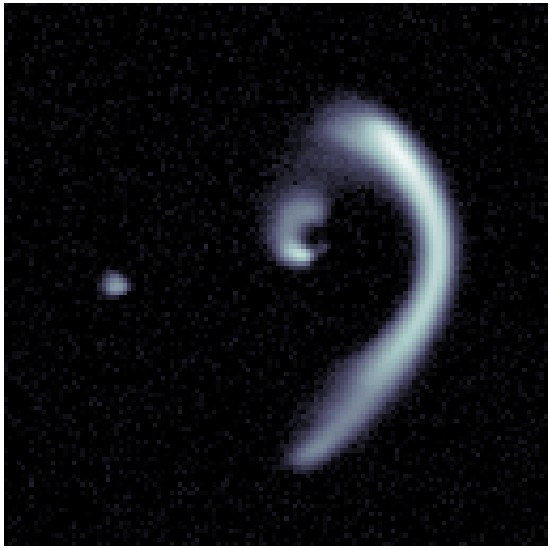
\includegraphics[width=2cm,height=2cm]{lens}};
        \node[text=white] at (-8.6, 2.2) {$\mathbf{y}$};
        \node[node, minimum width=4cm, minimum height=3cm] (x) at (1, 0) {};
        \node at (2.5, 1.8) {$\mathbf{\hat{x}}^{(t)}$};
        \node[rounded corners=.5cm, clip, inner sep=0] (source) at (2, 0) {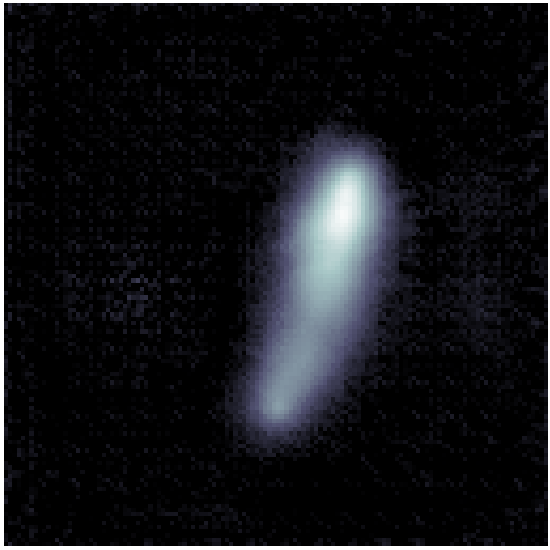
\includegraphics[width=2cm,height=2cm]{source_t2}};
        \node[text=white] at (1.6, -0.7) {$\mathbf{\hat{s}}^{(t)}$};
        \node[rounded corners=.5cm, clip, inner sep=0] (kappa) at (0, 0) {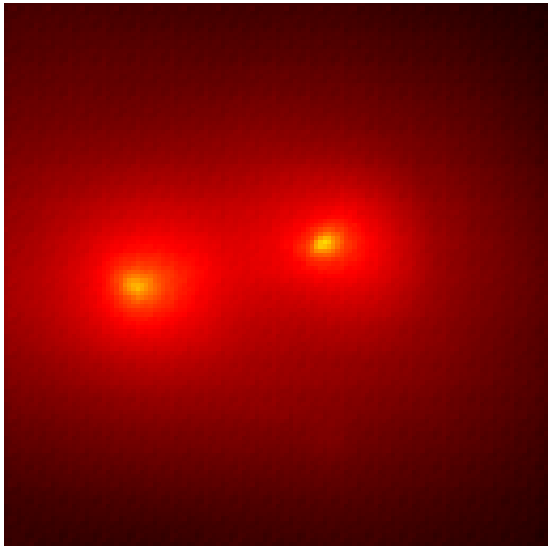
\includegraphics[width=2cm,height=2cm]{kappa_t2}};
        \node[text=white] at (-0.4, -0.7) {$\boldsymbol{\hat{\kappa}}^{(t)}$};

        \node[node] (F) at (1, -3) {Forward \\ Model};

        \node[rounded corners=.5cm, clip, inner sep=0] (obs_pred) at (-4, -3) {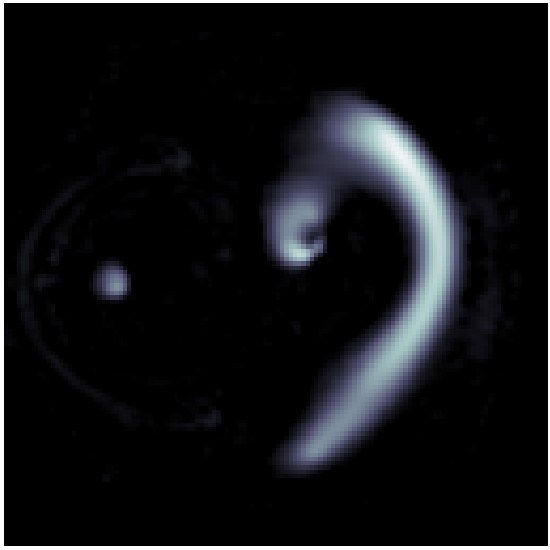
\includegraphics[width=2cm,height=2cm]{lens_t2}};
        \node[text=white] at (-4.4, -3.7) {$\mathbf{\hat{y}}^{(t)}$};

        \node[node] (rim) at (-4, 0) {Gradient \\ Update \\ $g_\varphi$};

        %\node[node] (grad k) at (-8.7, -3) {$\displaystyle \frac{\partial \chi^2}{\partial \boldsymbol{\hat{\kappa}}^{(t)}}$};
        %\node[node] (grad s) at (-7, -3) {$\displaystyle \frac{\partial \chi^2}{\partial \mathbf{\hat{s}}^{(t)}}$};
        \node[node] (likelihood) at (-8, -3) {$p(\mathbf{y} \mid \mathbf{\hat{x}}^{(t)})$};

        %\draw[-latex, thick, in=90, out=270] (source) to (F);
        %\draw[-latex, thick, in=90, out=270] (kappa) to (F);
        \draw[-latex, thick] (F) to (obs_pred);
        \draw[-latex, thick] (rim) to (kappa);
        \draw[-latex, thick] (obs_pred) to (likelihood);
        \draw[-latex, thick] (obs) .. controls +(-1, -2) and +(-1, 2) .. (likelihood);
        \draw[-latex, thick] (obs) .. controls +(0, -2.5) and +(-4, 0.5) .. (rim);
        \draw[-latex, thick] (likelihood) .. controls +(0, 2.5) and +(-4, -0.5) .. (rim);
        \node at (-7, -1) {$\grad_{\mathbf{y} \mid \mathbf{\hat{x}}^{(t)}}$};

        \draw[-latex, thick] (x) to (F);

        \draw[-latex, thick] (x) .. controls +(0, 3) and +(0, 3) .. (rim);

        %\draw[-latex, thick] (obs_pred) to (grad s);
        %\draw[-latex, thick] (grad s) .. controls +(0, 3) .. (rim);
        %\draw[-latex, thick] (grad k) .. controls +(0, 4) .. (rim);

        %\draw[-latex, thick] (source) .. controls +(0, 3) and +(-1, 3) .. (rim);
        %\draw[-latex, thick] (kappa) .. controls +(0, 2) and +(0, 2) .. (rim);

\end{tikzpicture}
\end{document}
